%% Ternary complex model
%% FigInline2EmergentSquares.tex
%% Unused packages and definitions removed; TikZ/PGFPlots source formatted.

\documentclass{standalone}

\usepackage{tikz}
\usetikzlibrary{arrows}

\def\b{\mathsf{b}}
\def\c{\mathsf{c}}
\def\d{\mathsf{d}}

\def\kappab{\kappa_{\b}}

\def\kappabp{\kappa_{\underline{\b}}}

\def\etabc{\eta_{\b\c}}
\def\etacd{\eta_{\c\d}}

\def\etabbp{\eta_{\b\underline{\b}}}

\def\etabc{\eta_{\b\c}}
\def\etacd{\eta_{\c\d}}

\begin{document}

\tikzset{every node/.style={minimum size=0.2cm,inner sep=2pt,outer sep=2pt}}

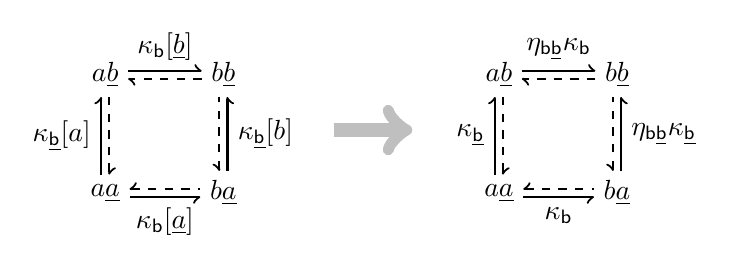
\begin{tikzpicture}[node distance=1.5cm]
    \begin{scope}[xshift=0cm]
        \draw (0,0) node (AAP) {$a\underline{a}$};
        \node[above of=AAP] (ABP) {$a\underline{b}$};

        \node[right of=AAP] (BAP) {$b\underline{a}$};
        \node[right of=ABP] (BBP) {$b\underline{b}$};
        \node[right of=ABP] (X) {};

        \draw[-left to,thick,transform canvas={xshift=-1.5pt}] (AAP) to node[left] {$\kappabp[a] $} (ABP);
        \draw[dashed,-left to,thick,transform canvas={xshift=1.5pt}] (ABP) to (AAP);

        \draw[dashed,right to-,thick,transform canvas={xshift=-1.5pt}] (BAP) to  (BBP);
        \draw[right to-,thick,transform canvas={xshift=1.5pt}] (BBP) to node[right] {$ \kappabp[b]$} (BAP);

        \draw[dashed,right to-,thick,transform canvas={yshift=1.5pt}] (AAP) to (BAP);
        \draw[right to-,thick,transform canvas={yshift=-1.5pt}] (BAP) to  node[below] {$\kappab[\underline{a}]$} (AAP);

        \draw[-left to,thick,transform canvas={yshift=1.5pt}] (ABP) to node[above] {$\kappab[\underline{b}] $} (BBP);
        \draw[dashed,-left to,thick,transform canvas={yshift=-1.5pt}] (BBP)to (ABP);
    \end{scope}

    \begin{scope}[xshift=2.9cm,yshift=0.8cm]
        \draw[->, line width=5pt, gray!50] (0,0) -- (1,0);
    \end{scope}

    \begin{scope}[xshift=5cm]
        \draw (0,0) node (AAP) {$a\underline{a}$};
        \node[above of=AAP] (ABP) {$a\underline{b}$};
        \node[above of=AAP] (Y) {};

        \node[right of=AAP] (BAP) {$b\underline{a}$};
        \node[right of=ABP] (BBP) {$b\underline{b}$};

        \draw[-left to,thick,transform canvas={xshift=-1.5pt}] (AAP) to node[left] {$\kappabp $} (ABP);
        \draw[dashed,-left to,thick,transform canvas={xshift=1.5pt}] (ABP) to (AAP);

        \draw[dashed,right to-,thick,transform canvas={xshift=-1.5pt}] (BAP) to  (BBP);
        \draw[right to-,thick,transform canvas={xshift=1.5pt}] (BBP) to node[right] {$ \etabbp \kappabp $} (BAP);

        \draw[dashed,right to-,thick,transform canvas={yshift=1.5pt}] (AAP) to (BAP);
        \draw[right to-,thick,transform canvas={yshift=-1.5pt}] (BAP) to  node[below] {$\kappab$} (AAP);

        \draw[-left to,thick,transform canvas={yshift=1.5pt}] (ABP) to node[above] {$\etabbp \kappab$} (BBP);
        \draw[dashed,-left to,thick,transform canvas={yshift=-1.5pt}] (BBP)to (ABP);
    \end{scope}
\end{tikzpicture}

\end{document}

